\subsection{Cenários energéticos e a matriz elétrica brasileira}
\begin{onehalfspace}
    O cenário energético mundial vem apresentando progressos quanto ao desenvolvimento da 
    eficiência energética e da busca de fontes limpas e renováveis de energia. A criação de 
    políticas de redução de consumo energético, assim como a promoção de congressos, eventos 
    e demais incentivos à pesquisa e desenvolvimento acadêmico apontam melhorias neste âmbito 
    da energia \cite{InternationalEnergyAgency-IEA2014}.\vspace{0.3cm} \newline
    Estudo desenvolvido pela \textcite{UnitedNations2017} aponta que 103 países definiram 
    a eficiência energética e uso de energias renováveis como parte importante do seu 
    planejamento estratégico, e destes, 79 são países emergentes e em desenvolvimento. 
    Constata-se, ainda, que o consumo de energia poderia ter sido 12\% maior em 2017 caso as 
    políticas públicas mencionadas anteriormente não tivessem sido implementadas desde o ano 
    2000 \cite{InternationalEnergyAgency-IEA2019b}.\vspace{0.3cm} \newline
    Entre os países emergentes e em desenvolvimento, nota-se que há um esforço para redução 
    de consumo de energia, o que reflete em fatores como o aumento da segurança energética, 
    aumento na competitividade industrial, redução de emissão de poluentes e da degradação 
    ambiental, expansão ao acesso de energia, além da indução ao crescimento econômico 
    \cite{BancoMundial2018}. Entretanto, de acordo com \textcite{Abramovay2010,Abramovay2014}, 
    a matriz energética mundial ainda será predominantemente composta por fontes fósseis de 
    energia até meados do século XXI.\vspace{0.3cm} \newline
    No Brasil, a taxa de consumo energético, assim como em outros países, é definida pelo 
    aquecimento econômico e cenários estabelecidos para o desenvolvimento esperado para o país. 
    Nesse sentido, espera-se que o Brasil, até 2026, apresente crescimento econômico e, 
    concomitantemente, consuma energia de forma modesta. Projeta-se que este crescimento seja 
    da ordem de 1,9\% ao ano até a metade da década analisada, com variações que definem o 
    crescimento do consumo em 2,3\% anuais, indicando otimismo para o setor de energia 
    brasileiro \cite{EmpresadePesquisaEnergetica-EPE2017,EmpresadePesquisaEnergetica-EPE2017a}.\vspace{-0.6cm}\newline \enlargethispage{0.25\baselineskip}
    
    \begin{graph} \label{g1}
        \par \small Gráfico 1 - Oferta interna de energia elétrica no Brasil (a) e a participação setorial de consumo de eletricidade (b).
        \begin{minipage}[ht]{1\textwidth}\centering
            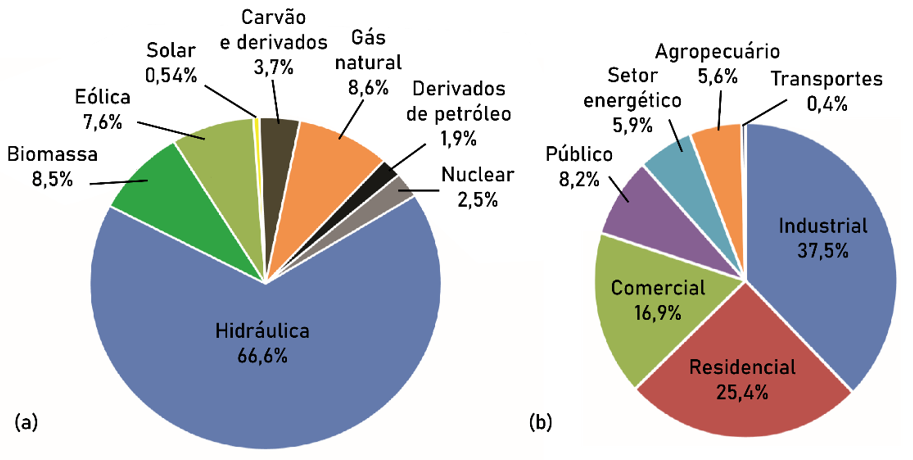
\includegraphics[width=0.7\textwidth]{graphs/graph1.png}            
        \end{minipage}
        \par \small Fonte: adaptado de EPE (2019).
    \end{graph}\pagebreak
    
    \noindent Em 2018, a geração hídrica respondeu por 66,6\% da oferta interna entre as fontes de
    produção de energia elétrica no Brasil, seguido do gás natural, com 8,6\%, da biomassa, 
    com 8,5\% e de outras fontes, 16,3\%, como mostrado no Gráfico 1. Deste modo, 
    as centrais hidráulicas de serviço público e de autoprodução contribuíram para expansão 
    da capacidade total instalada de geração de energia elétrica, com acréscimo de 3.864 MW 
    dos 5.728 MW, ou 67,5\% do total adicionado \cite{EmpresadePesquisaEnergetica-EPE2019}.\vspace*{0.3cm} \newline

    \noindent Esta contribuição para a expansão energética, além da representação na oferta interna de 
    energia elétrica, demonstra a importância da fonte para o país. Entretanto, fontes renováveis 
    de energia elétrica, como a solar e a eólica, representam uma alternativa a momentos de 
    condição desfavorável para oferta hídrica, como registrado em 2017, quando foi verificada 
    queda de 3,4\% da energia hidráulica disponibilizada em relação ao ano anterior \cite{EmpresadePesquisaEnergetica-EPE2018}.\vspace{0.3cm} \newline
    A representatividade nacional da fonte solar na geração de energia elétrica aumentou em 316,1\% 
    entre os anos de 2017 e 2018, crescendo de 832 GWh para 3.431 GWh. A potência instalada solar 
    fotovoltaica atingiu 1.798 MW em 2018, 47,99\% potência a mais disponível em relação ao ano 
    anterior, com 935MW \cite{EmpresadePesquisaEnergetica-EPE2019,EmpresadePesquisaEnergetica-EPE2019a}.\vspace{0.3cm} \newline
    Vale ressaltar o avanço na oferta de energia elétrica proveniente de micro e mini geração 
    distribuída, saltando de 359 GW, em 2017, para 828 GW, em 2018, resultando em um aumento de 131\%. 
    A contribuição para este crescimento se deu majoritariamente pela energia solar, com 63,5\%, 
    enquanto as fontes hídrica, gás natural, eólica e outras fontes renováveis contribuíram, respectivamente, 
    em 19,1\%, 1,8\%, 1,7\% e 13,9\% \cite{EmpresadePesquisaEnergetica-EPE2019}.\vspace{0.3cm} \newline
    O entendimento sobre a matriz elétrica nacional e a disponibilidade de fontes de geração de 
    energia elétrica serve como importante base para a definição de medidas de produção de energia, 
    assim como para o balanço energético das edificações. Este mapeamento de fontes energéticas 
    indica a potencialidade de geração de energia descentralizada, reforçado pelo crescimento 
    no número de geradoras de energia solar fotovoltaica no país e pelo avanço da oferta de energia 
    elétrica oriunda de micro e mini geração distribuída \cite{EmpresadePesquisaEnergetica-EPE2019,EmpresadePesquisaEnergetica-EPE2019a,Pereira2017}.\vspace{0.3cm} \newline
    Assim, a utilização de fontes renováveis de energia representa um aspecto importante para as 
    edificações Zero Energy aplicadas ao cenário brasileiro. Visto que é significativo o potencial 
    de uso da energia solar como fonte de produção de energia renovável, este recurso pode resultar 
    em reduções importantes no consumo de energia para uma parcela de consumidores dos setores 
    industrial, residencial e comercial, com quase 79,8\% de participação no consumo de energia 
    elétrica, como apresentado no \textcolor{red}{Gráfico 1b} \cite{Cronemberger2012,EmpresadePesquisaEnergetica-EPE2019,Sorgato2018,Sudhakar2019}.\vspace{0.3cm} \newline
    A composição da matriz elétrica do Espirito Santo mostra que a predominância da geração de 
    energia elétrica por fonte é termelétrica, ou térmica de gases de processo, em 2018, com 35,10\%, 
    enquanto a parcela de participação da fonte hidrelétrica é de 24,72\% \cite{AgenciadeRegulacaodeServicosPublicosdoEspiritoSanto-ARSP2018}.\vspace{0.3cm} \newline
    A evolução na geração de energia elétrica aponta que as fontes renováveis de energia estão 
    regredindo em participação, como mostrado no \textcolor{red}{Gráfico 2} que entre os anos de 
    2009 a 2012, compunham mais da metade da geração de energia, e atualmente estão em um 
    patamar de 35\%.\vspace*{-0.4cm}
    \begin{figure}[ht]
        \centering
        \caption{\small Evolução da geração de energia elétrica por fonte renovável e não-renovável no Espírito Santo.}
        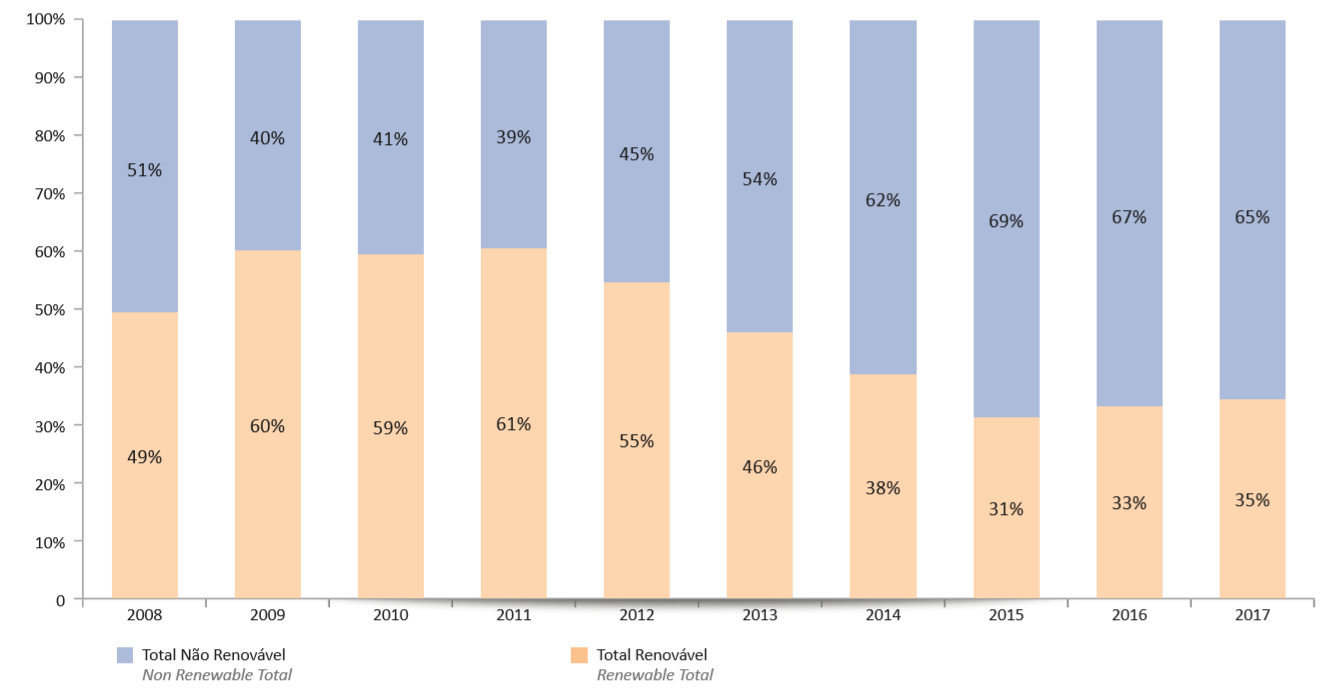
\includegraphics[width=0.8\textwidth]{graphs/graph2_geracao_de_energia_eletrica_no_es-arsp_2018.png}
        \begin{flushleft}
            \par \small Fonte: adaptado de ARSP (2018).
        \end{flushleft}
        \label{fig:Grafico 2}
    \end{figure}\newline
    \noindent O Espírito Santo conta ainda com a uma parcela geradora solar fotovoltaica, inaugurada em 2016 
    com capacidade de 1GW, de 2.820 usinas fotovoltaicas, configurando 28,8 MW de potência instalada 
    e geração de 8 GW \cite{AgenciadeRegulacaodeServicosPublicosdoEspiritoSanto-ARSP2018}.\vspace{0.3cm} \newline
    Observa-se que houve uma sensível variação no consumo de energia elétrica no Espírito Santo 
    entre os anos de 2016 e 2018. Houve o aumento de consumo das classes residencial e industrial, 
    compensado pela redução das classes comercial e rural, como observado no \textcolor{red}{Gráfico 3}. O consumo de 
    energia elétrica no Estado, em 2018, foi predominantemente da classe industrial, perfazendo 
    40,2\%, seguido pela classe residencial, com 24,1\%, comercial, consumindo 17,3\%, rural, 
    com 9,3\% e outros consumidores, com 9,1\% \cite{AgenciadeRegulacaodeServicosPublicosdoEspiritoSanto-ARSP2019}.
    
    \begin{figure}[ht]
        \centering
        \caption{\small Consumo de energia elétrica no Espírito Santo por classe.}
        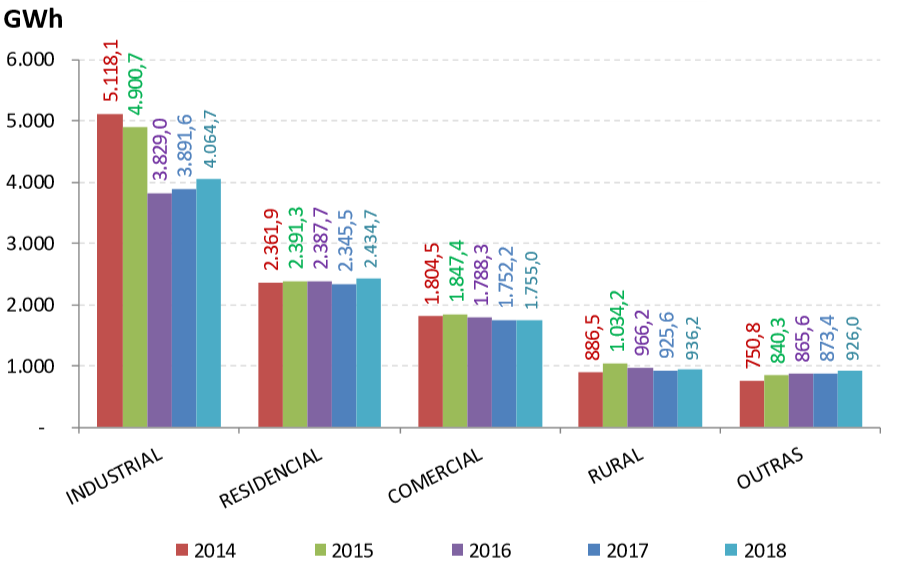
\includegraphics[width=0.7\textwidth]{graphs/graph3_consumo_de_energia_eletrica_no_es_por_classe-arsp_2019.png}
        \par \small Fonte: adaptado de ARSP (2019).
        \label{Grafico 3}
    \end{figure}\vspace*{-0.1cm}

    \subsubsection{Potencial de geração de energia solar no Brasil e no Espírito Santo}
    A avaliação do potencial de geração de energia estritamente solar se justifica, principalmente, 
    pela natural abundância do recurso disponível em território nacional \cite{Pereira2017}. Além 
    da disponibilidade de energia solar, a versatilidade da tecnologia fotovoltaica para adaptar-se 
    ao meio urbano e a redução de custo de instalação e manutenção são fatores importantes que 
    tornam a tecnologia acessível em detrimento de outras formas de geração de energia provenientes 
    de fontes renováveis, tais como a eólica, a geotérmica, a maremotriz, a biomassa, entre outras 
    \cite{AgenciadeRegulacaodeServicosPublicosdoEspiritoSanto-ARSP2019,Didone2014,Didone2014a,InternationalEnergyAgency-IEA2019b,UnitedNationsEnvironmentProgramme-UNEP2019}.\vspace{0.3cm} \\
    A oferta de energia solar no país varia de acordo com a região analisada, dada as dimensões 
    continentais do país. Segundo \textcite{Pereira2017}, a região Nordeste apresentou a menor 
    variabilidade interanual de energia solar, indicando maior estabilidade na produção de energia 
    solar, com valores entre 5,39 e 5,59 kWh/m². Já a região Sudeste apresentou a maior variabilidade 
    interanual, com médias entre 4,97 e 5,11 kWh/m² entre os anos de 2005 e 2015. A abrangência deste 
    rendimento energético anual pode ser observada na Figura \ref{Figura 3}.

    \begin{figure}[ht]
        \centering
        \caption{\small Rendimento solar anual brasileiro.}
        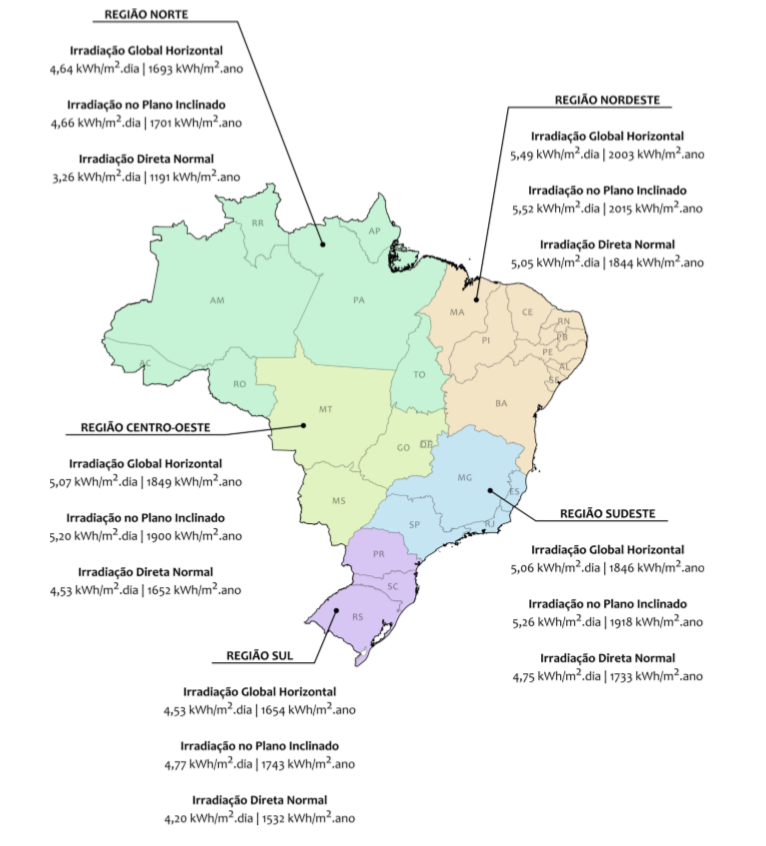
\includegraphics[width=0.9\textwidth]{figures/fig3-niveis_de_irradiacao_por_regiao_brasileira_pereira_et_al_2017.png}
            \begin{flushleft}
                \par \small Fonte: adaptado de Pereira et al. (2017).
            \end{flushleft}
        \label{Figura 3}
    \end{figure}\vspace*{-0.4cm}
    \noindent Os resultados de \textcite{Cronemberger2012}, após a conclusão do estudo em 78 cidade brasileiras, 
    apontaram que o Brasil é caracterizado como um país em baixa latitude e com alta disponibilidade 
    e uniformidade de radiação solar. Esta conclusão apontou a potencialidade das cidades brasileiras 
    para a geração de energia solar, tanto em superfícies planas como nas coberturas quanto em superfícies 
    verticais como as fachadas.\vspace{0.3cm} \newline
    \textcite{Pereira2017} complementam acerca do potencial brasileiro em gerar energia solar. Os autores 
    mencionam que mesmo nos locais menos ensolarados do Brasil, como as regiões Sul e Norte, apresentadas 
    na Figura \ref{Figura 4}, é possível gerar mais eletricidade solar do que no local mais ensolarado da Alemanha, 
    país com maior parque solar do mundo. As regiões Sul e Norte brasileiras recebem menos irradiação 
    solar por apresentarem as latitudes mais altas e, assim, com maiores diferenças entre a duração do dia; 
    e nebulosidade frequente, reduzindo a irradiância solar na superfície receptora. Isto indica a 
    característica do país para a produção de energia solar.\vspace{0.3cm}
    \begin{figure}[ht]
        \centering
        \caption{\small Mapa do total anual de irradiação solar direta normal.}
        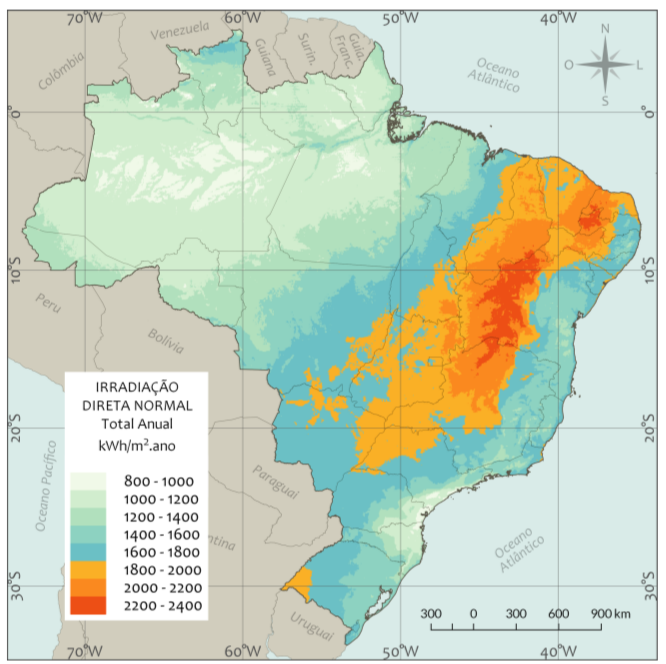
\includegraphics[width=0.85\textwidth]{figures/fig4-mapa2.png}
        \begin{flushleft}
            \par \small Fonte: adaptado de Pereira et al. (2017).            
        \end{flushleft}
        \label{Figura 4}
    \end{figure}\vspace*{-0.4cm}

    \noindent Outro ponto importante no estudo de \textcite{Pereira2017} foi a constatação de que a geração máxima 
    nos estados da região Sudeste, nos meses de verão, coincide com os máximos de demanda registrados 
    pelo Operador Nacional do Sistema – ONS, para a mesma região. Esta coincidência entre gerações 
    máximas de energia elétrica pode aliviar os períodos de pico de demanda de energia elétrica no país.\vspace{0.3cm} \newline
    \noindent O Espírito Santo gerou cerca de 8 GW de energia elétrica proveniente de energia solar em 2018. 
    Esta geração foi realizada por empreendimentos particulares, visto que o estado não abriga usinas 
    solares cadastradas junto ao SIN \cite{EmpresadePesquisaEnergetica-EPE2019a}. O estado também 
    apresenta variação no nível de radiação menor do que em estados com maior produção de energia solar 
    como a Bahia, com variação de 6,5 kWh/m²/dia \cite{AgenciadeServicosPublicosdeEnergiadoEstadodoEspiritoSanto-ASPE2013}.\vspace{0.3cm} \newline
    A Região Metropolitana da Grande Vitória – RGMV, em particular Vitória, apresenta variação baixa, 
    entre 5,39 a 5,48 kWh/m²/dia, como exposto na Figura \ref{Figura 5}. Esta variação indica que a geração de 
    energia elétrica pode ser melhor aproveitada em comparação a outros estados com maior potência 
    instalada \cite{AgenciadeServicosPublicosdeEnergiadoEstadodoEspiritoSanto-ASPE2013}.\vspace*{-0.63cm}
    \begin{figure}[ht]
        \centering
        \caption{\small Radiação solar no plano inclinado do ES.}
        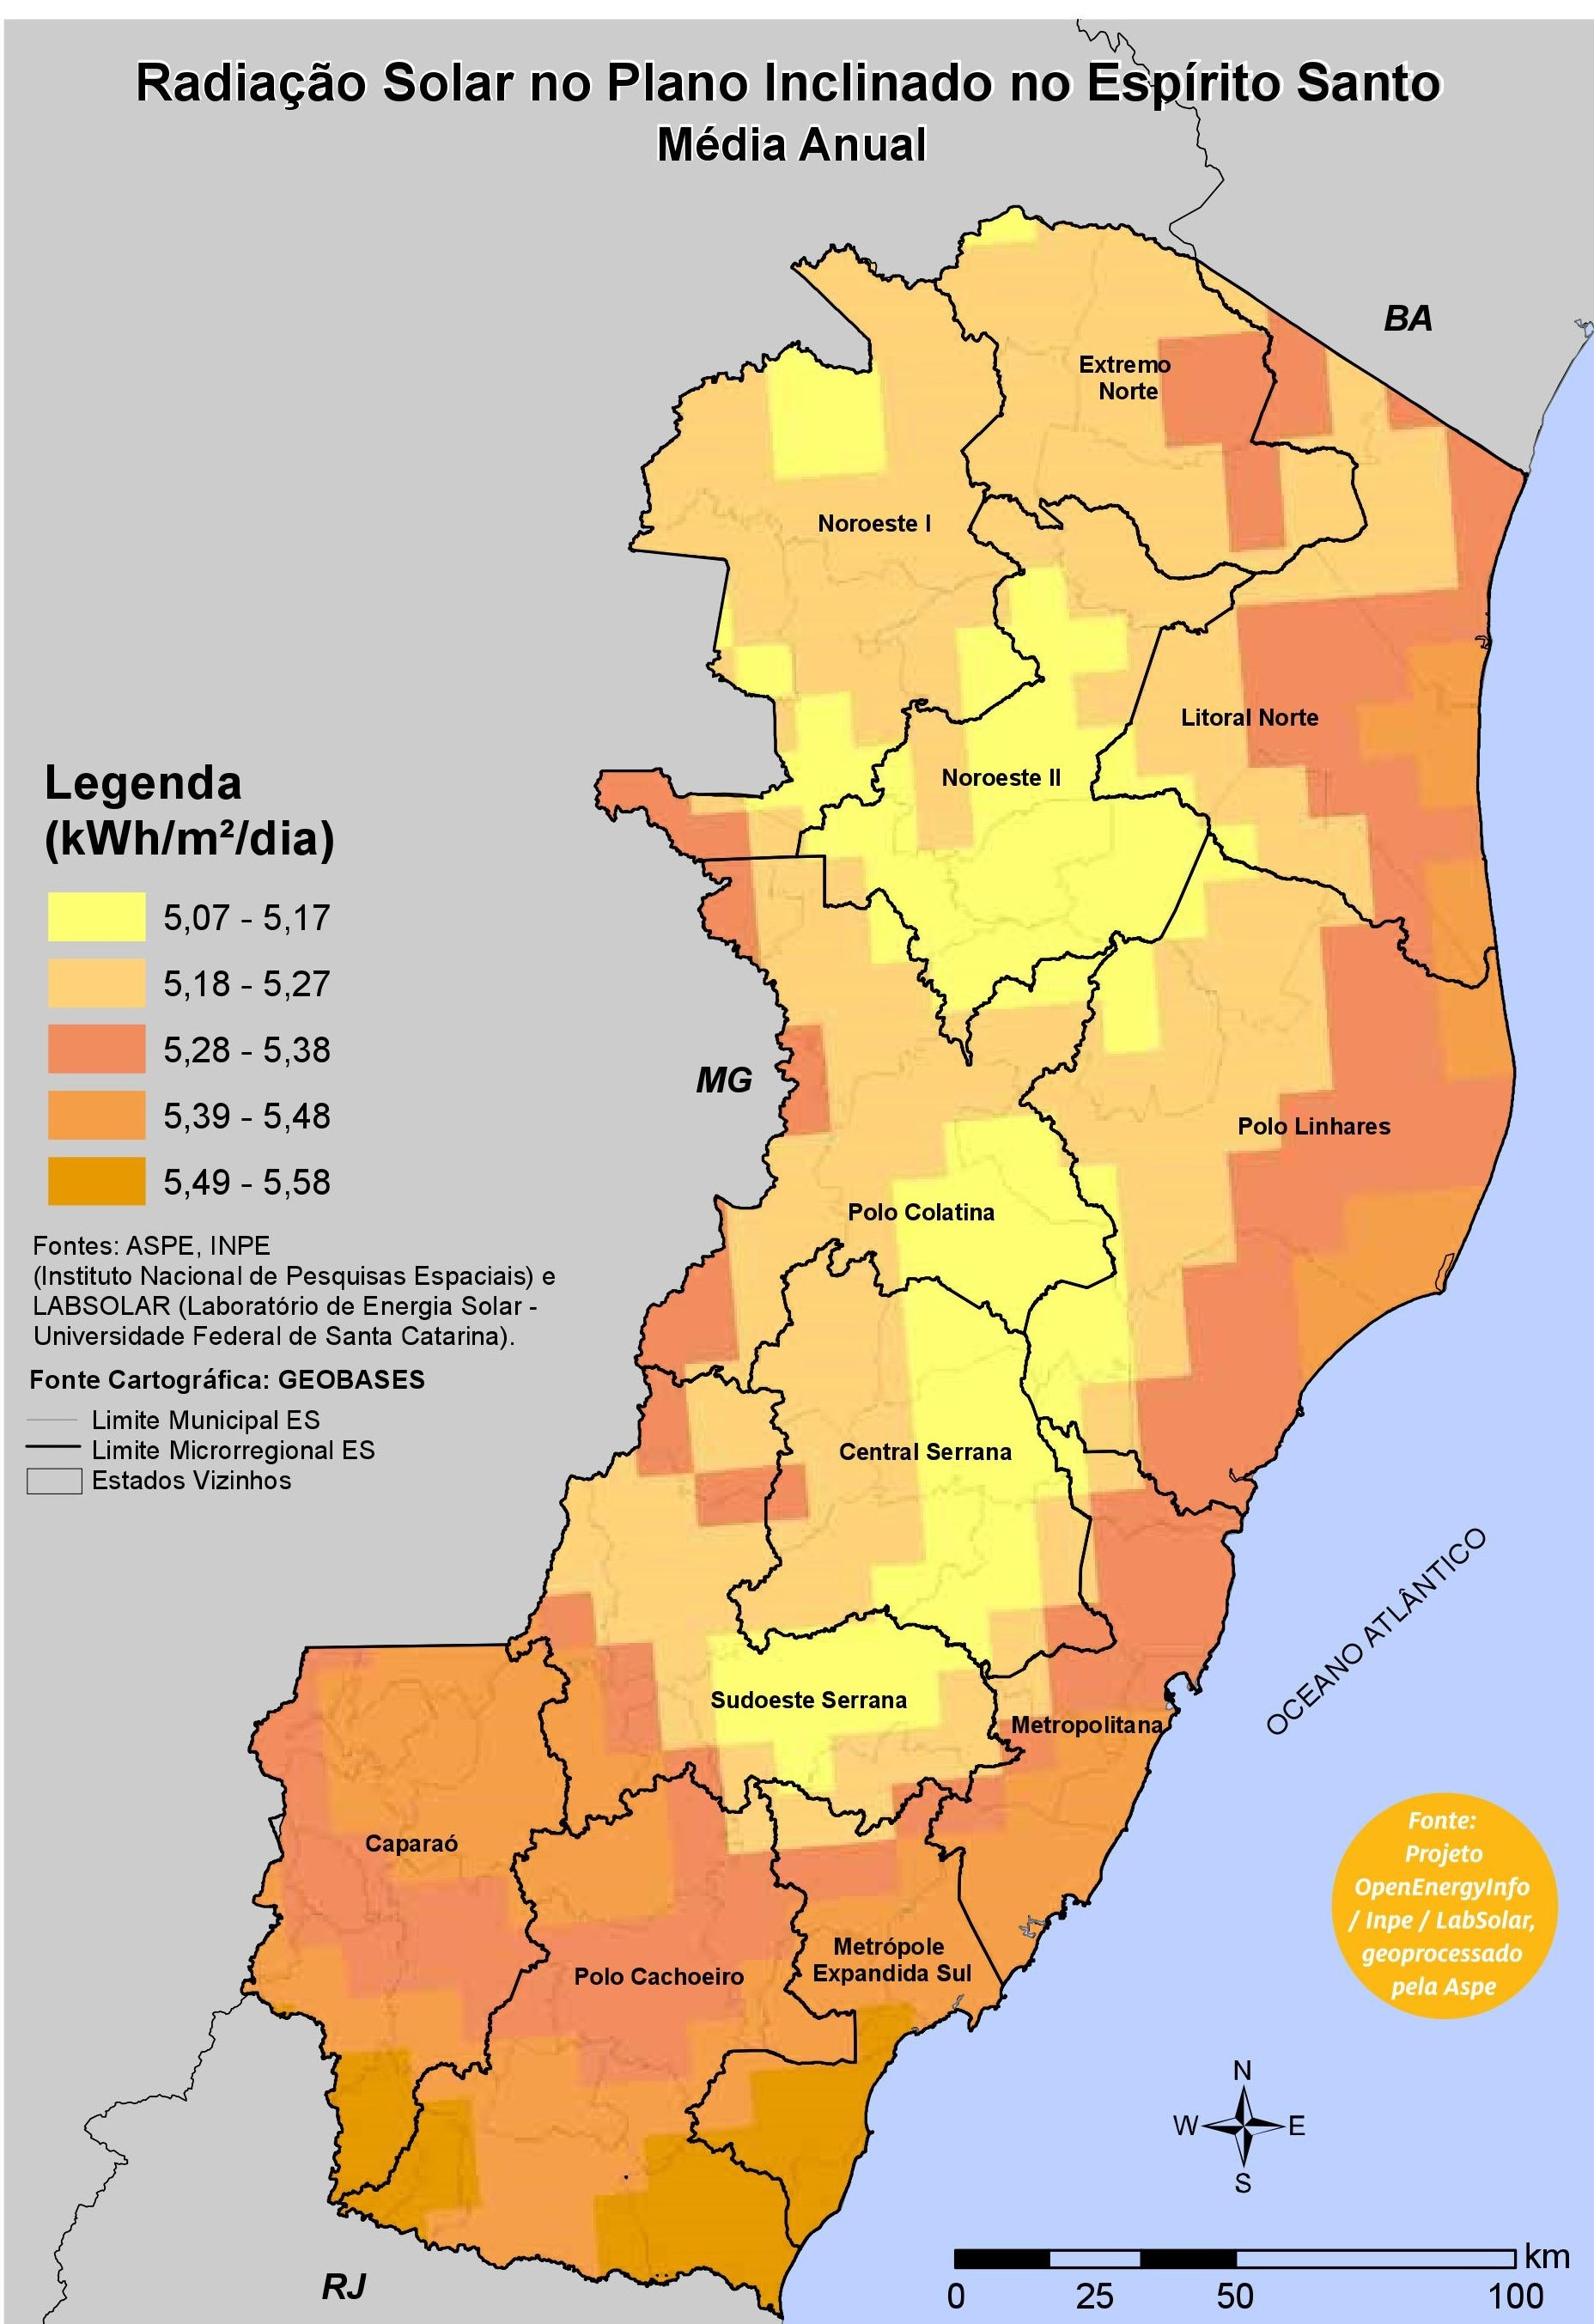
\includegraphics[width=0.55\textwidth]{figures/fig5-mapa3.jpg}
        \begin{flushleft}
            \par \small Fonte: adaptado de ARSP (2013).
        \end{flushleft}
        \label{Figura 5}
    \end{figure}

    \subsubsection{Energia solar fotovoltaica}
    As tecnologias de geração de energia fotovoltaica vêm evoluindo ao longo dos últimos anos. 
    Este segmento está em pleno crescimento quando observado o acesso técnico e econômico ao sistema de 
    geração de energia à população \cite{Pereira2017}. Equipamentos fotovoltaicos são fonte promissora 
    de diversidade em produção de energia, dada a versatilidade de aplicação e integração entre 
    sistemas para a envoltória da edificação \cite{Sorgato2018}.\vspace{0.3cm} \newline
    A geração de energia elétrica por meio de células fotovoltaicas ocorre pela conversão de radiação 
    incidente sobre a área da célula em uma diferença de potencial entre suas extremidades. Esta célula 
    é constituída por duas camadas de elementos semicondutores dopados positiva e negativamente, 
    normalmente silício, o que propicia o ordenamento da corrente de elétrons, como exemplificado na 
    Figura \ref{Figura 6}.

    \begin{figure}[ht]
        \centering
        \caption{\small Esquema de geração de energia por célula fotovoltaica.}
        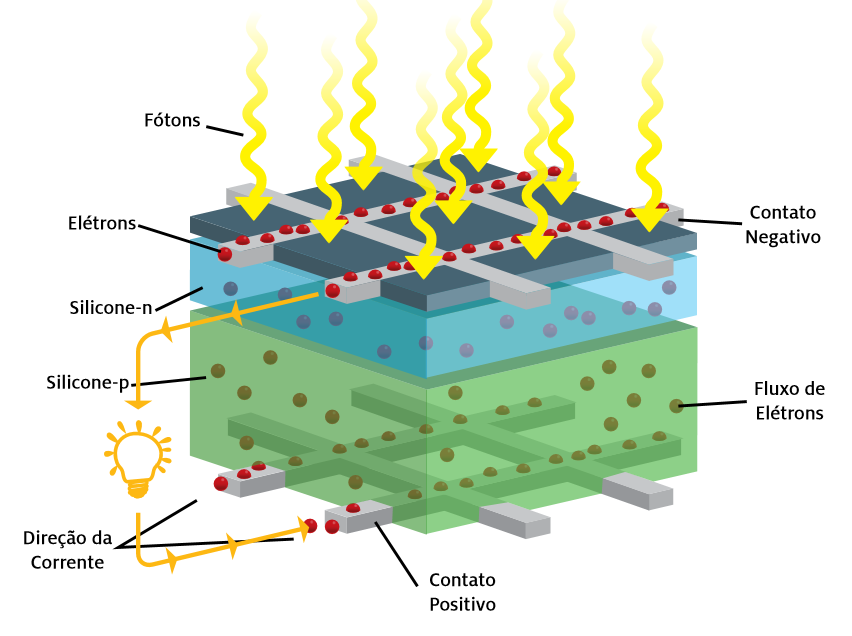
\includegraphics[width=1\textwidth]{figures/fig6_geracao_de_conrrente_continua_em_celulcas_fotovoltaicas_ARSP_2018.png}
        \begin{flushleft}
            \par \small Fonte: adaptado de ARSP (2013).
        \end{flushleft}
        \label{Figura 6}
    \end{figure}\vspace*{-0.4cm}
    \noindent Desde 1883, quando a primeira célula fotovoltaica foi constituída, a eficiência de conversão das 
    células avançou, partindo de 1\% a uma taxa de 19\% para os módulos comercializados atualmente. 
    Além da eficiência, o custo desta tecnologia foi barateado, aumentando o potencial de acesso pela população. 
    Os custos para a implementação da tecnologia saíram de US\$ 100/Wp, no início da década de 1970, 
    até US\$ 0,39/Wp, em 2016 \cite{AgenciadeServicosPublicosdeEnergiadoEstadodoEspiritoSanto-ASPE2013,Pereira2017}.\vspace{0.3cm} \newline
    Uma vantagem atribuída à aplicação de tecnologias fotovoltaicas na envoltória é a relação direta 
    entre quantidade de área de fachada exposta à radiação solar e a quantidade em potencial de produção 
    de energia solar fotovoltaica \cite{Veloso2017}. Outro fato importante é a verificação da viabilidade 
    econômica em climas tropicais como as cidades brasileiras apresentam \cite{Didone2014,Sorgato2018}.\vspace{0.3cm} \newline
    A versatilidade alcançada pela tecnologia é verificada pela facilidade de adaptação das células 
    fotovoltaicas para envoltória das edificações. Os componentes fotovoltaicos integrados ao edifício, 
    ou \textit{Building Integrated Photovoltaic} – BIPV, e os componentes fotovoltaicos adicionados/anexados a 
    edificação, ou \textit{Building Added/Attached Photovoltaic} – BAPV, são formas de introdução das 
    células para aproveitar a área disponível de fachada para produção de energia elétrica 
    \cite{AmericanSocietyofHeatingRefrigeratingandAir-ConditioningEngineers-ASHRAE2019}, como apresentado 
    pela Figura \ref{Figura 7}.\vspace*{-0.4cm}
    \begin{figure}[ht]
        \centering
        \caption{\small Componentes fotovoltaicos integrados a fachada do edifício Boulder Commons, localizado em Boulder, Colorado (EUA).}
        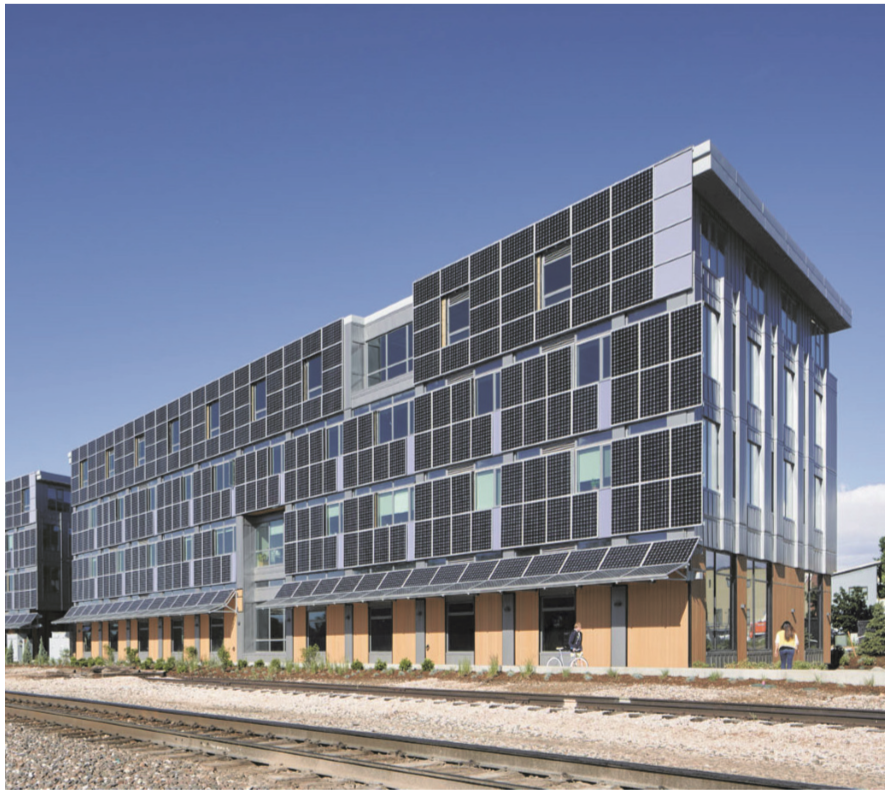
\includegraphics[width=0.75\textwidth]{figures/fig7_BIPV_ASHRAE_ZEB_2019.png}
        \begin{flushleft}
            \par \small Fonte: adaptado de ASHRAE (2019).
        \end{flushleft}
        \label{Figura 7}
    \end{figure}%\vspace*{-0.4cm}

    \noindent As edificações recebem a radiação solar de acordo com a latitude e a orientação solar onde estão situadas. 
    Estas características influenciam diretamente na produção de energia fotovoltaica de um painel, onde a 
    inserção dos painéis depende da orientação das superfícies das células fotovoltaicas voltadas para a posição 
    perpendicular em relação a latitude do local. Este posicionamento tende a maximizar a incidência de radiação 
    sobre as células e, assim, a produção de energia. Regiões com diferentes latitudes tendem a apresentar 
    variabilidades de fotoperíodo, onde as baixas latitudes geram menos energia com os painéis posicionados 
    verticalmente e mais energia para os posicionados horizontalmente, sendo que o inverso aplica-se às regiões 
    com altas latitudes \cite{Pereira2017}.\vspace{0.3cm} \newline
    No exemplo da Figura 7, o edifício comercial \textit{Boulder Commons}, localizado em Boulder, Colorado, 
    exemplifica a utilização de um sistema BIPV para geração de energia solar fotovoltaica em uma região de 
    alta latitude, com a utilização de painéis posicionados horizontal e verticalmente \cite{AmericanSocietyofHeatingRefrigeratingandAir-ConditioningEngineers-ASHRAE2019,Pereira2017}.
    Dentre as tecnologias de células fotovoltaicas disponíveis no mercado, destacam-se as tecnologias de 
    silício cristalino e filmes finos. As caraterísticas gerais desses componentes são apresentadas na Tabela \ref{tab:tabela1}.
    \begin{table}[ht]\centering
        \caption{\small - Tecnologias de células fotovoltaicas.}
        \vspace*{0.2cm}
        \label{tab:tabela1}
        \begin{tabular}{lcc}
        \hline
        \textbf{Tecnologia}                     & \textbf{Média anual total}    & \textbf{Área/kWp} \\ \hline
        \multicolumn{3}{l||}{Silício cristalino}                                                    \\ \hline
        Monocristalino                          & 20,67                         & ~8m²              \\ \hline
        Policristalino                          & 29,00                         & ~7m²              \\ \hline
        \multicolumn{3}{l||}{Filmes finos}                                                          \\ \hline
        Silício amorfo (a-SI)                   & 76,92\%                       & ~15m²             \\ \hline
        Telureto de cadmio (Cd-Te)              & 181,04                        & ~10m²             \\ \hline
        Disseleno de cobre-índio-gálio (CIGS)   & 2,05                          & ~10m²             \\ \hline
        \end{tabular}
        \begin{flushleft}
            \par \small Fonte: ARSP (2013).
        \end{flushleft}
    \end{table}\vspace*{-0.3cm}

\subsubsection{Legislação para a eficiência energética}
As políticas adotadas internacionalmente demonstram a urgência na busca de soluções relacionadas 
à mitigação do consumo de energia e redução de emissão de GEE, além de buscar, também, a redução 
dos impactos ambientais indiretamente relacionados ao ambiente construído \cite{InternationalMonetaryFund-IMF2018,InternationalEnergyAgency-IEA2018a}.\vspace{0.3cm} \newline
A Diretiva Europeia EPDB/31 (2010) estabeleceu como meta o balanço energético próximo a zero para 
novas edificações até dezembro de 2020. Nos Estados Unidos, o \textit{\textcite{U.S.DepartmentofEnergy-USDOE2015}}
apresentou medidas e programas para balanço energético nulo para as edificações comerciais e residenciais. 
O Departamento definiu como meta alcançar o balanço energético nulo em edificações residenciais 
até 2020 e edificações comerciais até 2025. Novas edificações comerciais, a partir de 2015, deveriam 
apresentar um plano de redução de energia desde sua concepção.\vspace{0.3cm} \newline
No Brasil, desde outubro de 2003 o Programa Nacional de Eficiência Energética em Edificações – 
PROCEL EDIFICA \cite{Brasil2001,Brasil2001a} atua de forma conjunta com o poder público, privado e a comunidade 
acadêmica para promover o uso racional da energia elétrica e recursos naturais em edificações. 
Nesta pesquisa, este marco legal foi utilizado como critério temporal de seleção para as edificações 
em Vitória concluídas após o início do programa, sendo então estabelecido o recorte temporal de 
estudos para edificações construídas após 2003.\vspace{0.3cm} \newline
Outro marco legal importante para o contexto desta pesquisa foi a Resolução Normativa nº 687 de 2015, 
substituindo a resolução precedente nº 482 de 2012, que trata sobre micro e mini geração de energia 
elétrica. Este conceito consiste em uma central geradora de energia elétrica que utilize fontes 
renováveis, com potência instalada superior a 75 kW e/ou capacidade instalada menor que 3 MW, 
classificado como mini geração; e potência instalada menor ou igual a 75 kW, classificado como 
micro geração \cite{AgenciaNacionaldeEnergiaEletricaANEEL2015}.\vspace{0.3cm} \newline
Com a regulamentação de micro e mini geração em território nacional, foi viabilizada a geração de 
energia descentralizada, característica importante para a coprodução de energia para uma edificação 
com balanço energético nulo.\vspace{0.3cm} \newline
Posteriormente, a Instrução Normativa nº 02 de 2014 institui a obrigatoriedade de submeter as edificações 
públicas ao Programa Brasileiro de Etiquetagem – PBE EDIFICA. Da mesma forma, foram criadas regulamentações 
relacionadas à eficiência energética e à certificações de edifícios de uso comercial e residencial, 
denominados Instrução Normativa Inmetro para a Classe de Eficiência Energética de Edificações Comerciais, 
de Serviços e Públicas, INI-C, e Instrução Normativa Inmetro para a Classe de Eficiência Energética 
de Edificações Residenciais, INI-R \cite{Dalbem2017,InstitutoNacionaldeMetrologiaNormalizacaoeQualidadeIndustrial-INMETRO2018}.\vspace{0.3cm} \newline
Os níveis de eficiência estabelecidos pelo regulamento partem do mais eficiente, classificado como 
“A”, para o menos eficiente, classificado como nível “E”. O regulamento classifica por meio de uma 
etiqueta indicativa do nível de eficiência energética da envoltória da edificação, dos sistemas de 
iluminação artificial e de condicionamento de ar \cite{InstitutoNacionaldeMetrologiaNormalizacaoeQualidadeIndustrial-INMETRO2018a}.\vspace{0.3cm} \newline
Dada a abrangência de cenários do regulamento e a utilização de referências como normas nacionais 
e internacionais para o desenvolvimento dos parâmetros de avaliação, o INI-C foi adotado como 
ferramenta de qualificação da eficiência energética e otimização dos modelos genéricos apresentados 
na etapa de metodologia. Esta escolha foi baseada na proximidade das características construtivas 
e de materiais sugeridas pela Instrução Normativa à realidade brasileira, sendo este fator pouco 
presente ou inexistente nas normas e regulamentos avaliadas.
\end{onehalfspace}